\documentclass[11pt, oneside]{article} 	% use "amsart" instead of "article" for AMSLaTeX format
\usepackage{geometry} 		% See geometry.pdf to learn the layout options. There are lots.
\geometry{letterpaper}  		% ... or a4paper or a5paper or ... 
\usepackage[parfill]{parskip} 		% Activate to begin paragraphs with an empty line rather than an indent
\usepackage{graphicx}				% Use pdf, png, jpg, or eps§ with pdflatex; use eps in DVI mode
								% TeX will automatically convert eps --> pdf in pdflatex		
\usepackage{amssymb}
\usepackage{amsmath}
\usepackage{authblk}
\usepackage[
backend=biber,
style=alphabetic,
]{biblatex}
\usepackage{graphicx}
\graphicspath{ {./images/} }
\usepackage{verbatim}
\usepackage{tikz} 
\usepackage{subcaption}
\captionsetup{compatibility=false}



\usepackage{syntonly}

% \syntaxonly \langle -- use this for checking syntax only
% \mbox {text} - keep together
% \fbox {text} - keep together and draw around

%\pagestyle{plain|headings|empty} % header and footer p.27
%SetFonts
%\include{filename}, \includeonly{filename1, filename2} , \input[fiename}

%SetFonts% 


\title{Dinosaur War: A Strategic Game of Utter Chance}
\author{Dave Fetterman}
\affil{Obviously Unemployed}
\date{2/238/23}
\begin{document}
\maketitle

\begin{abstract}

TODO 

\end{abstract}

\section{Pieceyard}


\begin{figure}
\centering
\begin{subfigure}{.5\textwidth}
  \centering
  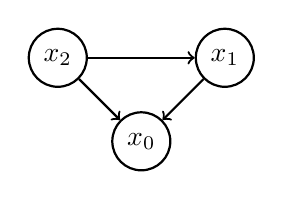
\begin{tikzpicture}[node distance={15mm}, thick, main/.style = {draw, circle}] 
\node[main] (1) {$x_0$}; 
\node[main] (2) [above right of=1] {$x_1$}; 
\node[main] (3) [above left of=1] {$x_2$}; 
\draw[->] (3) -- (2); 
\draw[->] (3) -- (1);
\draw[->] (2) -- (1);
\end{tikzpicture}
  \caption{($\mathbf{x_2}-x_1)(\mathbf{x_2}-x_0)(\mathbf{x_1}-x_0) \rightarrow x_2^2x_1^1x_0^0$}
  \label{fig:sub1}
\end{subfigure}

\begin{subfigure}{.5\textwidth}
  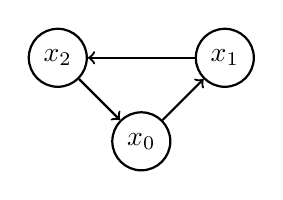
\begin{tikzpicture}[node distance={15mm}, thick, main/.style = {draw, circle}] 
\node[main] (1) {$x_0$}; 
\node[main] (2) [above right of=1] {$x_1$}; 
\node[main] (3) [above left of=1] {$x_2$}; 
\draw[<-] (3) -- (2); 
\draw[->] (3) -- (1);
\draw[<-] (2) -- (1);
\end{tikzpicture}

  \caption{($x_2-\mathbf{x_1})(\mathbf{x_2}-x_0)(x_1-\mathbf{x_0}) \rightarrow x_2^1x_1^1x_0^1$}
  \label{fig:sub2}
\end{subfigure}

\begin{subfigure}{.5\textwidth}
  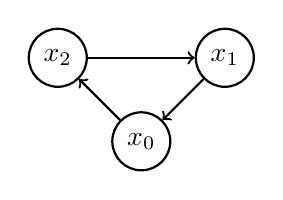
\begin{tikzpicture}[node distance={15mm}, thick, main/.style = {draw, circle}] 
\node[main] (1) {$x_0$}; 
\node[main] (2) [above right of=1] {$x_1$}; 
\node[main] (3) [above left of=1] {$x_2$}; 
\draw[->] (3) -- (2); 
\draw[<-] (3) -- (1);
\draw[->] (2) -- (1);
\end{tikzpicture}

  \caption{($\mathbf{x_2}-x_1)(x_2-\mathbf{x_0})(\mathbf{x_1}-x_0) \rightarrow -x_2^1x_1^1x_0^1$}
  \label{fig:sub3}
\end{subfigure}


\caption{Three terms of  $P_{[0,2]}$, corresponding to complete directed graphs of size 3}
\label{fig:test}
\end{figure}




\begin{center}
\begin{tabular}{||c c c c||} 
 \hline
t & $t \cdot g$ & Matching factor $t^*$ $\cdot$ Matching $g^*$ & First cycle \\ [0.5ex] 
 \hline\hline
 $x^4$ & $x^4d^3c^2b^1a^0$ & none & none  \\ 
 \hline
 $-x^3a$ & $-x^3d^3c^2b^1a^1$ & $-x^3b \cdot -d^3c^2a^1b^0$ & $(x,b,a)$ \\ 
 \hline
 $-x^3b$ & $-x^3d^3c^2b^2a^0$ & $-x^3c \cdot -d^3b^2c^1a^0$ & $(x,c,b)$ \\ 
 \hline
 $-x^3c$ & $-x^3d^3c^3b^1a^0$ & $-x^3d \cdot -c^3d^2b^1a^0$ & $(x,d,c)$ \\ 
 \hline
 $-x^3d$ & $-x^3d^4c^2b^1a^0$ & none & none \\ 
 \hline
 $x^2ba$ & $x^2d^3c^2b^2a^1$ & $x^2ca \cdot -d^3b^2c^1a^0$ &  $(x,c,b)$ \\ 
  \hline
 $x^2ca$ & $x^2d^3c^3b^1a^1$ & $x^2da  \cdot -c^3d^2b^1a^0$ &  $(x,d,c)$ \\ 
 \hline
 $x^2da$ & $x^2d^4c^2b^1a^1$ & $x^2db  \cdot -d^3c^2a^1b^0$ &  $(x,b,a)$ \\ 

 \hline
 $x^2cb$ & $x^2d^3c^3b^2a^0$ & $x^2db  \cdot -c^3d^2b^1a^0$ &  $(x,d,c)$ \\ 
 \hline
 $x^2db$ & $x^2d^4c^2b^2a^0$ & $x^2dc  \cdot -d^3b^2c^1a^0$ &  $(x,d,c)$ \\ 
 
 
\hline
 $x^2dc$ & $x^2d^4c^3b^1a^0$ & none &   none \\ 
 
 \hline
 $-xcba$ & $-xd^3c^3b^2a^1$ & $-xdba  \cdot -c^3d^2b^1a^0$ &  $(x,d,c)$ \\ 

 \hline
 $-xdba$ & $-xd^4c^2b^2a^1$ & $-xcba  \cdot -d^3b^2c^1a^0$ &  $x,c,b)$ \\ 

 \hline
 $-xdca$ & $-xd^4c^3b^1a^1$ & $-xdcb  \cdot -d^3c^2a^1b^0$ &  $(x,b,a)$ \\ 

 \hline
 $-xdcb$ & $-xd^4c^3b^2a^0$ & none &  none \\ 
 
 
 \hline
 $dcba$ & $ d^4c^3b^2a^1 $ & none &  none \\ 
 
 \hline
\end{tabular}
\end{center}

This sum, $x^4d^3c^2b^1a^0-x^3d^4c^2b^1a^0+x^2d^4c^3b^1a^0-xd^4c^3b^2a^0+d^4c^3b^2a^1$, when added to the tables of all the other initial settings of $g$, produces $S_{[0,4]}$.


\begin{thebibliography}{9}
\bibitem{1}
Wikipedia: \url{https://en.wikipedia.org/wiki/Minimax_theorem}
\end{thebibliography}


\end{document}

